\documentclass[10pt]{IEEEtran} 
\usepackage{graphics}
\usepackage[cmex10]{amsmath}

\setlength{\topmargin}{0pt}
\setlength{\headheight}{0in}
\setlength{\headsep}{0in}
\setlength{\textheight}{9.0in}
\setlength{\footskip}{0.5in}
\setlength{\oddsidemargin}{0pt}
\setlength{\evensidemargin}{0pt}
\setlength{\textwidth}{6.5in}

\begin{document}
\title{Scheduling Simultaneous Events for Multiple Mobile Devices}
\author{Jacob Schwartz}
\maketitle

\begin{abstract}
Computers keep their own time, which needs to be synchronized when communicating
over a network. Synchronizing the clocks on these networked machines helps fix
various potential problems but can also be used to schedule simultaneous events
on multiple smartphones or other mobile devices.  When working with two mobile
devices, one will act as the time source and the other will then synchronize to
it by calculating an offset. In this paper, a basic network time synchronization
technique will be used to schedule two mobile devices to take a picture at the
same time, according to one of the devices. We were successful in taking photos
on two iPhones hundredths of a second apart. This difference may be even less,
we need to find a more accurate testing tool.
\end{abstract}

\section{Introduction}

Applications that communicate to other machines over the Internet occasionally
need to have their times synchronized to create a reference point that would be
used for the rest of their communications.  Mobile phone applications may not
want to use their local clock in various instances. For example, a user may
change their local clock in order to beat a loophole in a game. In this case,
the phone would be comparing what it believes the time to be with a server. This
technique of time synchronization is not restricted to a client and a cloud
server, it can also be performed between two mobile clients on the same network.
In this instance, one of the devices will have to act as the ``server'', and the
other device will calculate its offset based on the ``server'' device's time,
even if it not the correct time.

In this paper, we use a basic process to calculate the time offsets between two
mobile devices. We schedule an event on one of the devices and it tells the
other device to schedule the same event for the same time, using the time offset
of the device. To show the these events occur at the same point in time, both
device take a picture of the same clock. To take the experiment a step further,
the scheduling of events could also take place across different platforms or run
off different wireless protocols like TCP or Bluetooth.

To calculate the offset, a formula similar to the one used in NTP will be used.
This involves taking the time three on three occasions. The client devices
checks its time when it sends the request packet to the service device. This
time will be called $t_0$. When the server receives the request packet, it
immediately send the client the time on the server's clock($t_1$). The last
time($t_2$) is recorded by the client when it receives $t_1$ from the server. 
It is assumed that the round trip time is symmetric. The offset($o$) is the
server time minus the client time minus the half of the round trip time:
\begin{equation}
    o = t_1 - t_2 - \frac{t_2 - t_0}{2} 
\end{equation}

\section{Results}

To test the validity of our algorithm, we wrote a simple application to find 
the offset between two mobile devices, iOS devices in this case. This
application has one device declare itself the server. This device then waits for
a client device to connect. Over a UDP connection, the server then sends the
device's time in milliseconds since the Unix Epoch several times, which the
client uses to get an average offset from its time. Once this offset is
calculated, the user tells the server device when to take a picture. The server
device then tells the client when it wants the picture taken, and it calculated
when it should take the picture using the offset. To determine how far off the
picture event take place, the phones are positioned to take a picture of a
digital stopwatch.

\begin{figure}
{\resizebox{3.2in}{!}{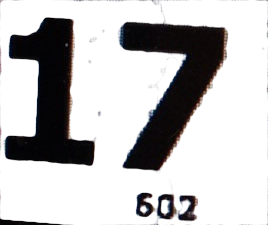
\includegraphics{experiment/jake.png}}}
\caption{Picture taken from ``Server'' phone}
\label{fig:pic0}
\end{figure}

\begin{figure}
{\resizebox{3.2in}{!}{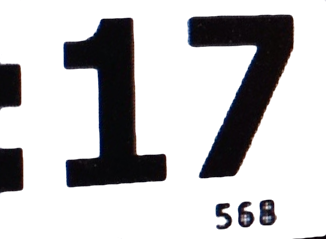
\includegraphics{experiment/radim.png}}}
\caption{Picture taken from ``Client'' phone}
\label{fig:pic1}
\end{figure}

\section{Conclusion}

This experiment was run between two iPhone 5 running iOS 7. As shown in figures
1 and 2, the time between the pictures was only four hundredths of a second, or
four nanoseconds. For most applications, this delay is acceptable. The
milliseconds in the figure 1 were not visible until the photo was manipulated,
leaving us to believe that this test was not as accurate as possible. We used an
online stopwatch, which does not refresh the screen faster enough to get an
exact measurement. A mechanical stopwatch or a pocket watch is required to get an
accurate measurement of the milliseconds between pictures.

There are several expansions to this project. One next step is to port the
application to other mobile operating systems to find any other potential
pitfalls that would cause the offset and the timing to be incorrect. Connecting
over Bluetooth would eliminate the 'ugliness' of having to enter an IP address
to connect. To use more than two devices, a multicast protocol could be used and
one of the mobile devices would act as a server or an actual dedicated server
could be used. The latter would also remove the need to enter an IP address,
because it would be static. 

\end{document}
